\documentclass[12pt]{article}
\usepackage{wkrpt}
\begin{document}


\title{Analysis of Asynchronous Programming techniques in Ecommerce Application}
{
	Minted LLC.\\
	San Francisco, CA 94111
}
{
	\textbf{Prepared by}\\[2ex]
	
	Daiwei Fan\\
	Student ID: 20458752\\
	User ID: d3fan\\
	4A Software Engineering\\
	May 1, 2016
}


\letter{Analysis of Asynchronous Programming techniques in Ecommerce Application}{third}{3B}{Minted LLC.}
{
	\noindent
	Daiwei Fan\\
	\#48, 461 Beechwood Place\\
	Waterloo, ON\\
	N2T 2N8
}
{
	Minted is a ecommerce platform that sells customizable arts and designs. Their main product include wedding invitations, digital invitations, uniquely designed stationary items etc. I decided to write this report based on the various concurrent programming techniques used in Minted's ecommerce funnel.
}
{
	The following report performs an analysis on the use of asynchronous techniques in different phases of the ecommerce funnel. The correct usage of technique is the interest of many parties in the company. My report will be used as a minor suggestion to the engineering team who makes the final decision of code refactoring.
}
{
	I would like to thank my mentor Linus Mixson, co-worker James Wu and devops engineer Patrick Gilbert, all of whom provided valuable background knowledge and priceless guidance over the course of my internship.
}
{
	Daiwei Fan\\
	Student ID: 20458752\\[2ex]
	Encl.
}


\tocsection{Executive Summary}

The following report performs an analysis on the use of asynchronous techniques in different phases of the ecommerce funnel. Four examples will be given. For each example, the report will discuss in detail regarding the reasoning behind using the current asynchronous technique; the kind of technology used and the way the technology is used; and finally the overall efficiency of the implementation.\\

The four examples are: Email generator, email sending server, order fulfilment server and batch promo code generation tool. Background knowledge will first be provided regarding the four examples. Then each example will be discussed in detail based on the three criteria above.\\

At the end the conclusion will be drawn and recommendations are made. The conclusion roughly states that the use of the technologies are adequate but the choice of technologies could be improved in the future. Suggestions of improvement will be given in the recommendation section.\\


\newpage

\tableofcontents
\newpage
\listoffigures
\newpage


\pagenumbering{arabic}
\section{Introduction}

Minted is an online marketplace of independent artists and designers. "The company crowdsources art and graphic design through monthly challenges. The public votes for the winning entries, and Minted produces the winning work as stationery, wall art, and decor."\cite{mintedllc}. "In October 2014, Minted was named \#5 on LinkedIn's 10 Bay Area startups that are most in demand by local techies."\cite{mintedllc} In January 2016, I was assigned to the infrastructure team which oversees the high level engineering design of Minted's ecommerce funnel. In this funnel, there are several levels of interfaces that interacts with the user to customize their product and finally make the order. Over the course of my internship, I began to gain interest in the programming techniques used in this funnel. To ensure smooth and intuitive shopping experience, the use of asynchronous programming should be carefully applied.\\

\begin{figure}[ht!]
\centering
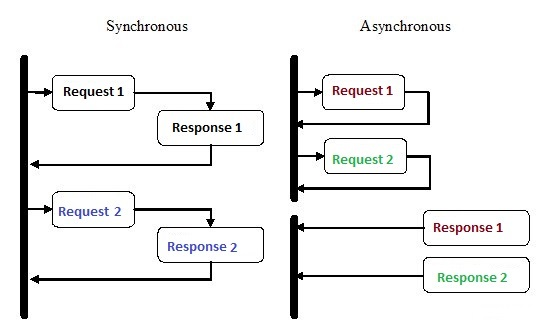
\includegraphics[width=12.5cm,height=12.5cm,keepaspectratio]{img/async.jpg}
\caption{Sync vs. Asynchronous programming}
\label{overflow}
\end{figure}

Nowadays asynchronous programming has become more and more popular. The benefit of concurrency it brings has increased the efficiency of millions of software. One of the reasons is that computer hardware has been built to perform concurrent tasks for more than a decades now, but on the software side it has only become widely popular in recent years. As a result, support for asynchronous programming are more often added to new technologies. Namely Python 3.x has a very powerful tool set for it. At Minted, different approaches have been used to implement asynchronous features. For example, for sending email campaigns to registered customers, generated emails are batched and a request is sent to a jobs client and queued. When it is the batch's turn to be processed, the jobs client will send the emails and makes a call back to a email campaign listener to acknowledge the success of sending the batch of emails.\\


This report provides an analysis of the use of asynchronous techniques in different places of the ecommerce funnel. For each use case, I will explain the purpose of applying the technique, the kind of technique applied, the way it is applied and comments of whether the application is efficient. Finally, the report summarizes the results of the analysis, draws conclusions, and makes a recommendation. The reader is expected to have reasonable background in web service development. Basic knowledge in python is a plus. Other technology and terminologies used in this report will be explained on their first appearance.\\



\newpage

\section{Problem Specification}
\subsection{Background}
Ecommerce funnel is a term used to describe the process of converting an anonymous person to a paid customer. The process consists of several steps including advertising/email campaign, site navigation/product selection, product customization, order placement and finally order processing. Following is an illustration of the ecommerce funnel.\\
\begin{figure}[ht!]
\centering
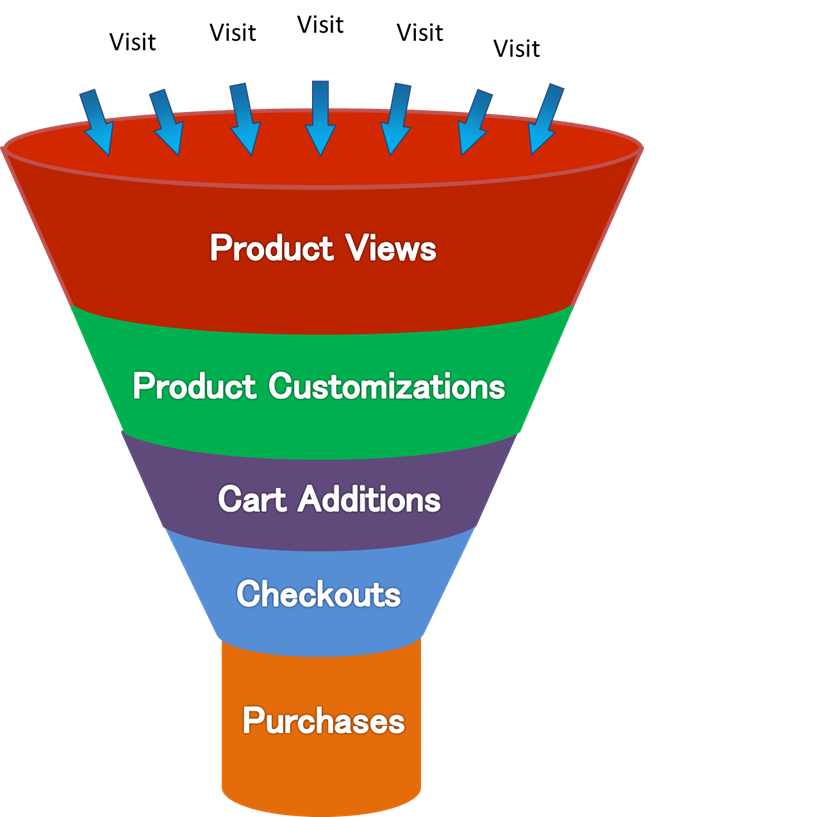
\includegraphics[width=12.5cm,height=12.5cm,keepaspectratio]{img/funnel.png}
\caption{Ecommerce funnel}
\label{overflow}
\end{figure}


\subsection{Options}
This report will be analysing the concurrent techniques used in the following phases of the funnel:
\subsubsection{Email campaign}
Minted sends automated emails to users periodically for advertising purposes. The emails often contain newsletters regarding new products, ongoing promotions or user exclusive coupons. The emails are generated by an automated campaign client and are batched to be sent via a third party email service provider called "Responsys".\\
		
\begin{figure}[ht!]
\centering

\includegraphics[width=5cm,height=5cm,keepaspectratio]{img/email-marketing.jpg}
\caption{Email marketing}
\label{overflow}
\end{figure}

\subsubsection{Order placement and processing}
This is the phase where the user has finished customizing their items and are ready to checkout. The typical step is to enter the billing and shipping address along with a valid credit card credential. Due to security commitements, Minted will not be saving the credit card information. Instead a third party credit card authentication service called "Cybersource" is used.\\

\subsubsection{Batch promo code generation tool}
As previously mentioned, Minted often sends user exclusive coupons via emails. This means the coupon code is tied to the user's account and no others can redeem it. As a result a mass number of coupons need to be created. I personally designed this tool for the sales department to conveniently create a large number of promo codes.\\
\newpage

\section{Analysis}
There are several aspects of an application of a programming technique that need to be analysed to judge if the technique is well applied. First of all the reasoning behind applying such technique. Secondly the kind of technology used and the way it is applied. Lastly the efficiency of the application compared to other alternatives.\\
\subsection{Email Campaign}

\subsubsection{Email Generator}
As briefly explained in the introduction, the way Minted sets up email campaign is by implementing a cron job that acts as an email generator. A cron job is a time-based job scheduler in Unix-like computer operating systems. People who set up and maintain software environments use cron to schedule jobs (commands or shell scripts) to run periodically at fixed times, dates, or intervals.\cite{cron} At Minted the generator is scheduled to run at the 30th minute of every hour. The reasoning behind using a cron job is very simple: the activation of the generator should be automated and it should run independent from the main web application. Obviously, having a sales employee trigger an email generation is silly since the rule to generate a single email for a single user can be pre-defined. For example, if Minted wants to send a shipping promotion to a user who has an item in his cart for longer than two days, than this rule could be normalized and coded into the email generator. The generator would thus filter the qualifying customers based on this logic. In addition, an email campaign is meant to be an advertisement that is sent to the user when his/she is not on the site. So it should be run in parallel along with the website.\\

In terms of the type of technology picked for the generator. Cron jobs are one of the most effective way of scheduling periodic tasks. Since it is built directly into any Unix machine, minimal setup work is required for virtually any types of server the company might be using. This is valuable when it comes to saving engineering and development operation costs.\\

Finally, the goal of parallel processing is achieved effectively. Currently Minted has roughly ten email generator instances running in parallel, each instance is created for a different campaign. Moreover, these generators will not block any process of the main web service which really showcases the beauty of asynchronous programming.\\

\subsubsection{Email Server}
Running a cron job to generate emails is only one of the two levels of asynchrony for email campaign. The generators are not responsible for sending the emails. Instead, they are batched and a request is sent to an email server. The batch of emails will be queued on the server and processed when the server is free. It is not difficult to comprehend the reason Minted wants an email server. Sending an actual email can take quite some time, the SMTP (Simple Mail Transfer Protocol) used to send emails is an old piece of technology. One of its greatest flaws is that it does not have a timeout restriction, so if a timeout is not set on the mail server, the connection could be hanging on a network problem and incoming emails can be indefinitely delayed. Even if a timeout is set, for example, Apache uses 60 seconds for the timeout, Microsoft uses 100 seconds,\cite{unit} \cite{maven} it can take quiet a while to send (or indicate a failure to send) a batch of 1000 emails should there be a network problem. As said in the previous section, an email generator for each campaign is set to run once every hour. But if by the next hour the previous generator for the campaign still has not terminated, two instances of the same campaign could be running at the same time. This could potentially cause unsent emails or duplicated emails. Queuing all the emails on a server can solve this problem elegantly.\\

\begin{figure}[ht!]
\centering
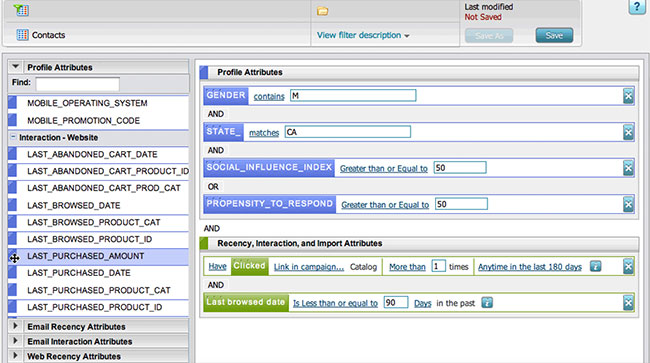
\includegraphics[width=12cm,height=10cm,keepaspectratio]{img/responsys.jpg}
\caption{Responsys interface}
\label{overflow}
\end{figure}

The reason Minted is picking a third party mail server is because building your own email server to achieve asynchronous mail delivering can be very costly. Responsys is an experienced and robust service that Minted has been using for 5 years. From the logs on the Responsys server, Responsys has a roughly 98\% success rate in sending emails. The sample is all the campaign emails sent through Responsys from the week of Apr. 11th, 2016. On the other hand, there is the minor problem that a mail server does not guarantee the quickness of sending an email. In the case of a network problem where there is a large number of emails being queued on the server, an email can be delayed for as much as several hours. After studying the business requirements, I believe that email campaigns are relatively less time sensitive. A rare case of long email delay can be tolerated and is one of the least concerns for a sales person.\\


\subsection{Order Placement}
Asynchronous processing has become the industry standard for ecommerce. When you buy something from online retailers, upon submitting your order, the website is most likely going to tell you that your order is submitted or completed, but it would not tell you that it is being processed. In this case, some kind of asynchronous processing has to be in place otherwise your web page would be hanging for hours until your order is processed. In short, the very nature of order fulfilment demands asynchronous programming application. The reasoning behind this is that a lot of things has to be done between the order placement and order shipment. And this part cannot be dealt with by adopting third party software since it contains too much business logic and Minted special services.\\

\begin{figure}[ht!]
\centering
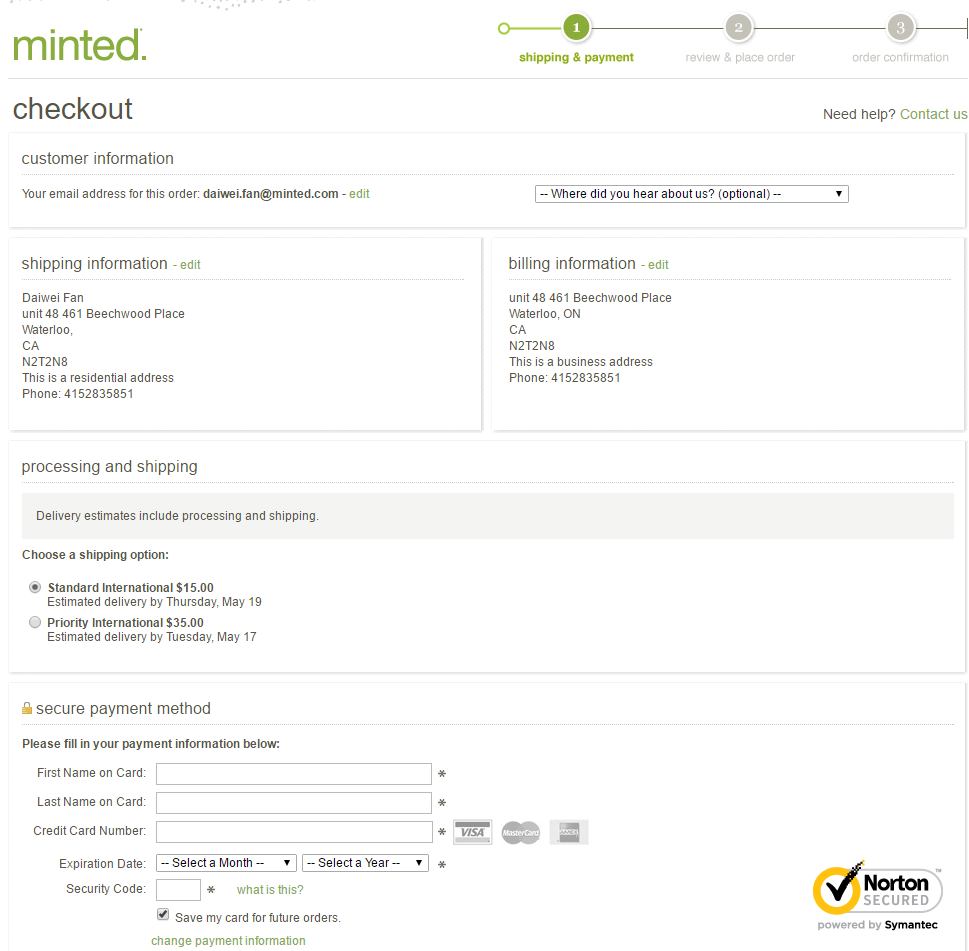
\includegraphics[width=15cm,height=20cm,keepaspectratio]{img/order.png}
\caption{Minted order confirmation page}
\label{overflow}
\end{figure}

At Minted, the biggest challenge to shrink the time of fulfilment is to address users special requests. Minted allows users to leave verbal instructions if the customization tool we provide is not powerful enough for the users. To tackle this challenge, Minted has implemented a fulfilment server that manages all submitted orders. Submitted orders are queued on the server similar to a batch of emails. These orders will first be verified with the third party credit card authentication service "Cybersource", to verify that payments have been received. Then, the orders are dispatched to the fulfilment crew to complete any special instructions. \\

Currently, there are noticeable flaws in the fulfilment server. It is common to see a large number of submitted orders queued on the server once or twice in a month. These are likely caused by existing bugs and extensive special instruction fulfilments. However, Minted is trying its best optimizing the server so that delay caused by non-human factors can be reduced to a minimum.\\


\subsection{Promo Code Generator}
As previously mentioned, I have created an internal tool for the sales crew to create large number of promo codes in a batch. One of the biggest challenge was to implement asynchrony to the tool. There are two reasons that asynchrony is necessary for this tool. The first one is that a user can be asking for a million promo codes. For every single code created, the tool will populate basic information about the code, for example, the promo code string and its id. Then, the tool will both write the information to database and to a CSV file for the user to download. This can take quite a bit of time if max write per second limit is taken into consideration (this maximum is used to protect the integrity of the hardware). Therefore the tool cannot be just waiting endlessly for the tool to finish. Secondly, the generated CSV is very large in size (roughly 5G for a million promo codes). The file is just not practical for any type of synchronous displaying methods, whether it's sending all the promo codes through an email or display all the codes on the tool's page.\\

I found that the asynchronous programming support for python 3 is perfect for this kind of task. Unfourtunately, after some consultation with engineers at Minted I found that python 3 was not currently supported and the cost would be impractical to support it along with python 3, not mentioning this is just for a small internal tool. Thus I was forced to use a cron job to implement the tool. The solution combines previously considered alternatives. After the user submits a promo generation request, the request will be queued as a database table entry. When the cron job is activated, the job will read through the table to find queued requests. The job will then create the promo codes and upload the generated CSV file to S3 server (an Amazon cloud based server). An email with the download link will be sent to the user to requested the codes.\\

Although it is foreseeable that this will be less efficient than the python 3 solution, this approach is still sufficient for the need of the sales crew. And through some rigorous testing the tool has proved its robustness and reliability.\\


\newpage
\section{Conclusions}
In conclusion, the use of asynchronous programming techniques in the above four places are overall reasonable. Especially for the fulfilment server, it is unrealistic to implement a synchronous service for order placement. Although this analysis lacks some quantitative evidence to prove the reasons are adequate, my conclusions have been agreed by several engineers at Minted. Especially for the batch promo generator, my work has been commended by many in the company.\\

The kind of technology used and the way they are used are adequate. The efficiency of the implementation isn't ideal but they are generally acceptable. For email generator, the goal of parallel processing is achieved effectively. The email server also has a satisfactory success rate. The fulfilment server still needs some improvements. And finally the batch promo generator is considered as robust and reliable. In other words, the use of the technologies are adequate but the choice of technologies could be improved in the future.\\

\newpage
\section{Recommendations}
For the Responsys mail server, a callback can be implemented from Responsys to a Minted email service listener to indicate that a particular email is sent. This will put Minted in a less dependent relationship with Responsys which currently gives the log report.\\

For the fulfilment server, further actions can be performed to reduce wait time after order placement. For example, for a digital product order, the dispatching process will be skipped and the user would be able to directly access the content they bought after credit card authentication. This could help catalysing the fulfilment process and moving the queue faster.\\

For the batch promo creation tool, it is recommended that a backend wide overhaul to take place to support python 3. This is the ultimate weapon that can provide with many elegant asynchronous solutions in the engineering design in the future.\\




\newpage


\addcontentsline{toc}{section}{\refname}
\bibliography{wkrpt}
\begin{thebibliography}{1}

  \bibitem{mintedllc} Minted LLC., "Minted: Home," Minted LLC., {\em http://www.minted.com/} (current April 11 2016).

  \bibitem{cron} Unix Geeks, "Newbie: Intro to cron" Unix Geeks, {\em http://www.unixgeeks.org/security/newbie/unix/cron-1.html} (current April 11 2016).

\bibitem{unit} Microsoft Corp., ".NET timeout" MSDN - Microsoft, {\em http://msdn.microsoft.com/en-us/library/aa292197(v=vs.71).aspx} (current April 11 2016).

\bibitem{maven} Apache Foundation., "Apeche SMTP timeout" Apache Foundation, {\em http://maven.apache.org/} (current April 11 2016).

\end{thebibliography}
\newpage


\tocsection{Acknowledgements}
I would like to thank my mentor Linus Mixson, co-worker James Wu and devops engineer Patrick Gilbert, all of whom provided valuable background knowledge and priceless guidance over the course of my internship.\\

\end{document}

